\documentclass{myslide}
\usepackage[listings,slide]{mypackage}

\title{C语言理论知识总览}
\subtitle{Week 17}

\author[chhzh123]{陈鸿峥}
\date[Dec, 2018]{December, 2018}

\keywords{}

\begin{document}

\begin{frame}
\titlepage
\end{frame}

\begin{frame}
\tableofcontents[subsectionstyle=show]
\end{frame}

\section{简介}
\begin{frame}
\sectionpage
\end{frame}

\begin{frame}{简介}
\begin{itemize}
	\item 一些有用的网站
		\begin{itemize}
			\item 题库 \url{https://www.sanfoundry.com/c-interview-questions-answers/}
			\item 在线测试 \url{https://rank.sanfoundry.com/c-programming-tests/}
			\item 问题 \url{https://stackoverflow.com/}
			\item 参考手册 \url{https://www.gnu.org/software/gnu-c-manual/gnu-c-manual.html}
			\item 圣书 K\&R Brian Kernighan and Dennis Ritchie, \emph{The C Programming Language}
		\end{itemize}
	\item 不会将C的所有理论知识点都讲完,只会选取一些重点、易忽视的点讲
\end{itemize}
\end{frame}

\section{为什么要学C}
\begin{frame}
\sectionpage
\end{frame}

\begin{frame}{TIOBE Ranking}
Dec 2018 Ranking
\begin{figure}
\centering
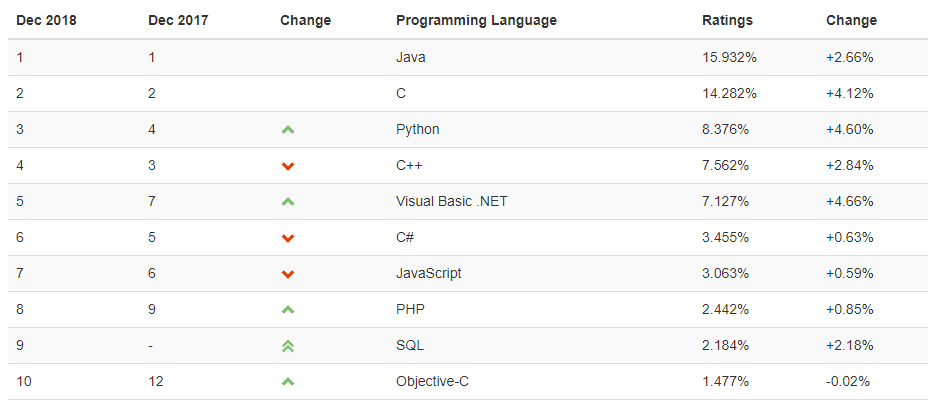
\includegraphics[width=\linewidth]{fig/TIOBE.PNG}
\end{figure}
\end{frame}

\begin{frame}{Why C Programming Language}
\begin{itemize}
	\item 速度、稳定性、可移植性 % cin
	\item 操作系统、嵌入式系统、驱动程序、底层操作
	\item 其他语言的编译器、库、解释器(Python、PHP、Perl)
	\item 科学计算(Mathematica、MATLAB)
\end{itemize}
\pause 然而
\begin{center}
C语言并不是必须的,\textbf{C++}应用范围更广也会更好用
\end{center}
\pause 然然而
\begin{itemize}[<+->]
	\item 学C++重点在于弄清楚如何面向对象编程(OOP)
	\item 千万不要将程序写得跟C一样(不是C with STL)
	\item 生活不只有ACM
\end{itemize}
\end{frame}

\section{知识点}
\begin{frame}
\sectionpage
\end{frame}

\subsection{计算机的基础知识}
\begin{frame}
\subsectionpage
\end{frame}

\begin{frame}{编译的四个阶段}
\begin{center}
\begin{tikzcd}
\text{源程序 hello.c}\arrow{d}{\text{预处理器(Preprocessor)}}\\% 宏的作用
\text{添加了宏的源程序 hello.i}\arrow{d}{\text{编译器(Compiler)}}\\
\text{汇编程序 hello.s}\arrow{d}{\text{汇编器(Assembler)}}\\
\text{可重定位目标程序 hello.o(bj) + printf.o}\arrow{d}{\text{链接器(Linker)}}\\
\text{可执行二进制程序 hello}
\end{tikzcd}
\end{center}
\end{frame}

\begin{frame}{一些易混淆的地方}
\begin{itemize}
	\item<1-> 解释器(Interpreter):直接执行高级语言(Python)
	\item<2-> 另外的编译体系(Java Virtual Machine, JVM)
	\begin{itemize}
		\item 字节码/中间码(byte code):包含执行程序,由一序列指令代码和数据组成的二进制文件
		\item 机器码/原生码(machine/native code):CPU可直接执行的代码,可执行二进制程序(executables)
	\end{itemize}
\end{itemize}
\end{frame}

\begin{frame}[fragile]{数的表示 - 进制(Number Systems)}
\begin{itemize}
	\item 十进制(decimal)
	\item 二进制(binary) \verb'0b'(整数除2、小数乘2)
	\item 八进制(octal) \verb'0'
	\item 十六进制(hexadecimal) \verb'0x'
\end{itemize}
举例:20=\verb'0b10100'=\verb'024'=\verb'0x14'
\end{frame}

\begin{frame}{数的表示 - 计算机的算术}
\begin{itemize}
	\item 原码(sign-magnitude):最高位为符号位
	\item 反码(\textbf{ones'} complement):原码按位取反
	\item 补码(\textbf{two's} complement):反码+1
\end{itemize}
\pause
* 浮点数
\begin{center}
\begin{tabular}{|c|c|c|}\hline
符号S,1 & 阶码E,8,移码 & 尾数F,23,原码
\\\hline
\end{tabular}
\end{center}
移码偏置常数为127(单精度)、1023(双精度)
\[(-1)^S\times1.F\times 2^{E-127}\]
\end{frame}

\begin{frame}{计算机编码}
\begin{itemize}
	\item ASCII (American Standard Code for Information Interchange)
	\begin{itemize}
		\item 7位或8位二进制数
		\item `0':48, `A':65, `a':97
	\end{itemize}
	\item Unicode (统一码/万国码/单一码) / UTF-8:为每种语言中的每个字符设定了统一且唯一的二进制编码,以满足跨语言、跨平台进行文本转换、处理的要求
\end{itemize}
\end{frame}

\subsection{变量}
\begin{frame}
\subsectionpage
\end{frame}

\begin{frame}{变量名}
\begin{itemize}
	\item<1-> 长度限定:任意长,但只会处理
	\begin{itemize}
		\item C89:$\leq 31$字符的内部标识符,$\leq 6$字符的外部标识符
		\item C99:$\leq 63$字符的内部标识符,$\leq 31$字符的外部标识符
	\end{itemize}
	\item<2-> 可用字符:大小写$52$+阿拉伯数字$10$+下划线$1$=$63$
	\item<2-> 组合规则:
	\begin{itemize}
		\item 第一个字符不可数字(也即可以是字母或下划线)
		\item 但避免\_开头,因操作系统和C标准库一般以\_开头(不是环境变量)
	\end{itemize}
	\item<3-> 关键字:全小写
	\item<3-> \textbf{可以}有相同的变量名与函数名,不会报错
\end{itemize}
\end{frame}

\begin{frame}[fragile]{局部变量与全局变量}
\begin{itemize}
	\item 局部变量:只在作用域内起作用
	\begin{itemize}[<+->]
		\item 最近的大括号对内,\verb'for'循环不写大括号也算
		\item 记得初始化,否则值为不确定的值
		\item 避免在函数内返回局部变量,主要是指针类型,如数组
	\end{itemize}
	\item 全局/外部变量:作用域由定义处开始到程序结束,用\verb'extern'修饰
	\begin{itemize}[<+->]
		\item 不跨文件在程序前文声明了,则可不写修饰符
		\item 全局变量自动初始化为0(数值型变量)、空字符(字符变量)
		\item \verb'extern'后面要不要加类型(如\verb'extern int i'),看不同版本编译器
	\end{itemize}
\end{itemize}
\end{frame}

\begin{frame}[fragile]{静态变量与自动变量}
\begin{itemize}
	\item 静态变量:\verb'static'\\
	在静态存储区分配存储单元,返回函数调用时值不会被清除,在程序整个运行期间都不释放
	\begin{itemize}
		\item 变量、函数、结构体全部都可以static
		\item 不可\verb'static static int'
	\end{itemize}
	\item 自动变量:\verb'auto'\\
	在动态存储区分配存储单元,每次函数调用新建,结束后即释放
	\begin{itemize}
		\item 没有加修饰词的都是自动变量,\verb'auto'可省略
		\item * 区别C++11中的auto关键字
	\end{itemize}
\end{itemize}
\end{frame}

\begin{frame}[fragile]{进程的内存分布(Memory Layout)}
\begin{columns}
\begin{column}{0.6\linewidth}
\begin{figure}
\centering
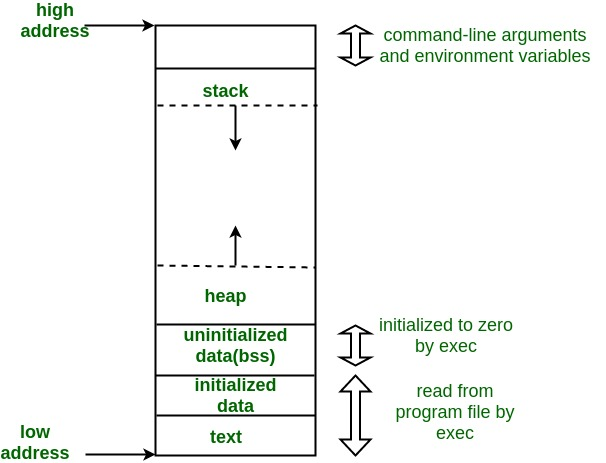
\includegraphics[width=\linewidth]{fig/memoryLayoutC.jpg}
\end{figure}
\end{column}
\begin{column}{0.4\linewidth}
\begin{center}
\textbf{数据和代码}都\\
\textbf{无区别}地用\textbf{二进制}存储
\end{center}
\end{column}
\end{columns}
\footnotetext[1]{\fontsm\url{https://www.geeksforgeeks.org/memory-layout-of-c-program/}}
\end{frame}

\begin{frame}[fragile]{进程的内存分布(Memory Layout)}
\begin{columns}
\begin{column}{0.4\linewidth}
\begin{figure}
\centering
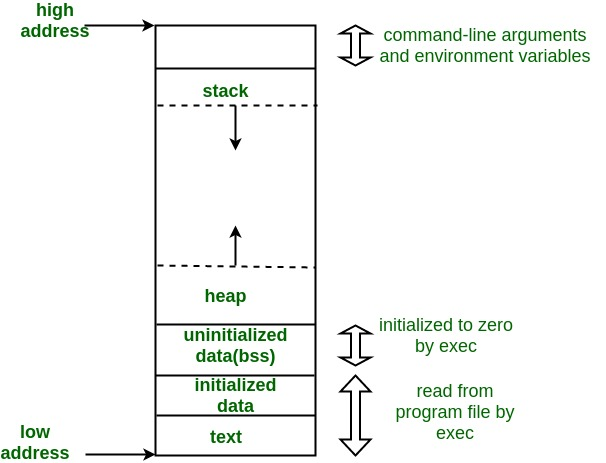
\includegraphics[width=1.1\linewidth]{fig/memoryLayoutC.jpg}
\end{figure}
\end{column}
\begin{column}{0.6\linewidth}
\begin{itemize}[<+->]
	\item 文本/代码(Code)段:包含可执行指令
	\item 数据(Data)段:包含\textbf{已初始化的全局变量、静态变量},并非只读区间
	\item BSS(Block Started by Symbol)段:\textbf{未初始化的全局变量、静态变量}
	\item 栈(Stack)段:先进后出,用于函数调用,包含\textbf{自动变量}
	\begin{itemize}
		\item 决定了你能开多大的局部变量、能递归函数多少次
		\item 栈段一般是8KB,开大数组一定要开全局!
	\end{itemize}
	\item 堆(Heap)段:动态内存分配,用\verb'malloc'、\verb'realloc'、\verb'free'管理
\end{itemize}
\end{column}
\end{columns}
\footnotetext[1]{\fontsm\url{https://www.geeksforgeeks.org/memory-layout-of-c-program/}}
\end{frame}

\begin{frame}[fragile]{定义与声明}
\begin{center}
\Large\verb'int i = 5;'\\
\verb'extern int i;'
\end{center}
\pause
\begin{itemize}
	\item 定义(definition):指编译器创建一个对象,为这个对象\textbf{分配}一块内存并取名(即变量名)
	\begin{itemize}
		\item 定义只可有一次
		\item C里没有\verb'string str'
		\item C99 \verb'for'循环内可定义变量
	\end{itemize}
	\item 声明(declaration):告知编译器这个名字已经匹配到一块内存上,并将这个名字和内存链接起来(没有分配内存)
	\begin{itemize}
		\item 声明可以出现多次
	\end{itemize}
\end{itemize}
\end{frame}

\begin{frame}[fragile]{定义与声明总结\protect\footnotemark}
\begin{center}
\begin{tabular}{|c|c|c|c|}\hline
 & 声明 & 定义 & 初始化\\\hline 
\verb'int i;'(局部)  &  Yes      &     Yes  &        No\\\hline
\verb'int i=5;'(局部)&  Yes      &     Yes  &       Yes (5)\\\hline
\verb'int i;'(全局)  &  Yes      &      No  &       Yes (0)\\\hline
\verb'extern int i;'  &  Yes      &      No  &        No\\\hline
\end{tabular}
\end{center}
\footnotetext[1]{\fontsm\url{https://stackoverflow.com/questions/4769599/declaration-or-definition-in-c}}
\end{frame}

\subsection{数据类型}
\begin{frame}
\subsectionpage
\end{frame}

\begin{frame}[fragile]{数据类型}
\only<1>{
\begin{figure}
\centering
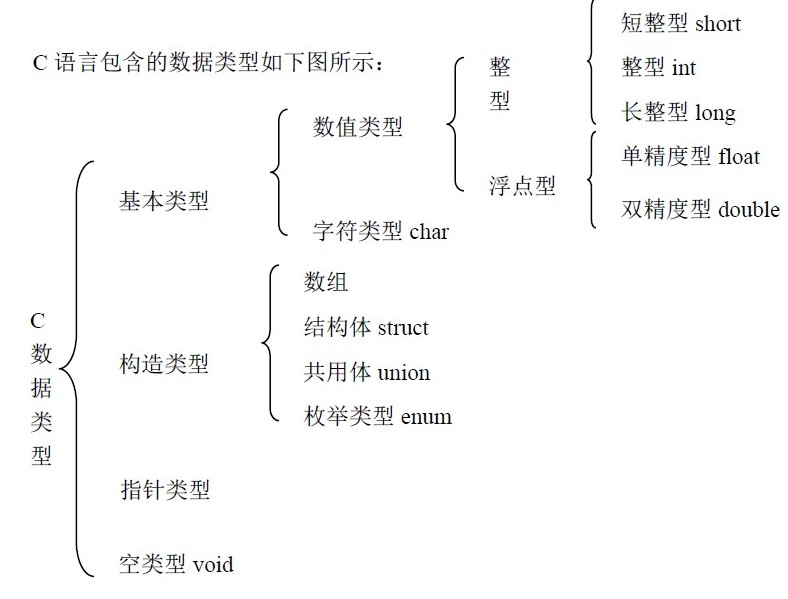
\includegraphics[width=0.8\linewidth]{fig/datatype.jpg}
\end{figure}
}
\only<2>{
\begin{itemize}
	\item enum:定义类型不占用空间,定义变量才占用
	\item short int:修饰符(qualifier)+基本数据类型(basic data type)
	\item float:无声明0.1默认为double,可以强行转换(0.1f)
\end{itemize}
}
\only<3->{
sizeof
\begin{itemize}
	\item \textbf{单目运算符}
	\item 返回类型的\textbf{字节}大小,由系统编译器决定
	\item 数组sizeof是数组元素sizeof之和,enum不表
	\item 特别注意区别struct和union
	\item 指针之后再讲
\end{itemize}
}
\only<4>{
1字节(Byte)=8位(Bit),故32位机是4字节
\begin{center}
\begin{tabular}{|c|c|}\hline
char & 1\\\hline
short & 2\\\hline
int & 4\\\hline
long & 4/8\\\hline
float & 4\\\hline
double & 8\\\hline
\end{tabular}
\end{center}
}
% \begin{lstlisting}
% float f1=0.1;
% f1==0.1f;
% \end{lstlisting}
\end{frame}

\begin{frame}[fragile]{数的表示}
\begin{itemize}[<+->]
	\item \verb'float x  %d' 出来垃圾值
	\item \verb'int x  %f' 出来为非常小的数,输出即为0
	\item \verb'char a  %d' 出来为ASCII码值
	\item \verb'int i=23 < char a=-23' 不一定,看编译器!
	\item \verb'unsigned int x=-5  printf("%d",x)' 仍为-5
\end{itemize}
\end{frame}

\begin{frame}[fragile]{常量}
\begin{itemize}
	\item 用\verb'const'进行修饰
	\item 常量必须初始化,否则编译错误
	\item \verb'\r'回车到行首(carriage return)
\end{itemize}
\end{frame}

\subsection{算术逻辑表达式}
\begin{frame}
\subsectionpage
\end{frame}

\begin{frame}[fragile]{算术 - 除法}
\begin{itemize}
	\item 不同语言对于除法的定义不一样!
	\item 除法\verb'/'在C里为\textbf{截断}(truncate)取整除法
	\item \textbf{整型}除以\textbf{整型}就是\textbf{整型},不会进行自动类型转换
\end{itemize}
% r=a-(a/b)*b为余数
e.g.\\
\[-9/4=9/-4=-2\qquad9/4=-9/-4=2\]
\end{frame}

\begin{frame}[fragile]{算术 - 自增}
\begin{itemize}
	\item \verb'++a + ++a'一定要有空格,但依然是未定义行为(Undefined Behavior, UB)
	\item \verb'sizeof(x++)'不会增加x的值\footnotemark[1]
\end{itemize}
\footnotetext[1]{\fontsm\url{https://stackoverflow.com/questions/8225776/why-does-sizeofx-not-increment-x}}
\end{frame}

\begin{frame}[fragile]{算术 - 逻辑}
\begin{itemize}[<+->]
	\item 逻辑与逻辑或都有\textbf{短路}运算,前者为0或1,可判断时将不会执行后续操作
	\item 0为假,非零值均为真;但逻辑表达式的返回值只会是0或1
	\item 按位取反\verb'~'包括符号位也要取反,故\verb'~0=-1'区别于\verb'!0=1'
	\item 移位,左移乘2,右移除以2(向下取整);注意对于有符号数来说是\textbf{算术}右移(符号位扩展)
\end{itemize}
\end{frame}

\begin{frame}[fragile]{算术 - 其他}
\begin{itemize}[<+->]
	\item 只有\verb'*= /= %= += -= <<= >>= &= |= ^='没有\verb'&&='
	\item 赋值表达式具有返回值,为赋值成功的值
	\item 连续赋值是合法的
	\item 一定看清是几个符号,是==还是=,是\&\&还是\&,并且注意\verb'for'循环后有无分号
	\item 注意缩进不是C语句的判断标准!
	\item 逗号表达式取最后一个运算得到的值
\end{itemize}
\pause
* if比较不会出错的写法是\verb'if(8 == x)'
\end{frame}

\begin{frame}[fragile]{运算优先级}
{\Large\textbf{单算移关与,异或逻条赋}}
\begin{columns}
\begin{column}{0.5\linewidth}
\begin{itemize}
	\item \verb'() ['index\verb'] -> .'
	\item 单目运算符(右结合) \verb'++ -- sizeof & * !'(逻辑非) \verb'~'(按位反) \verb'-'(负号)
	\item 算术\verb'* / %'
	\item \verb'+ -'
	\item 移位\verb'<< >>'
	\item 关系\verb'> < >= <='
	\item \verb'== !='
	\item 按位与\verb'&'
\end{itemize}
\end{column}
\begin{column}{0.5\linewidth}
\begin{itemize}
	\item 按位异或\verb'^'
	\item 按位或\verb'|'
	\item 逻辑与\verb'&&'
	\item 逻辑或\verb'||'
	\item 条件(三目运算符)\verb' ? :' 
	\item 赋值\verb'+= -= ='
	\item 逗号\verb','
\end{itemize}
\quad\\
*p++相当于*(p++)右结合
\end{column}
\end{columns}
\end{frame}

\subsection{控制流}
\begin{frame}
\subsectionpage
\end{frame}

\begin{frame}[fragile]{循环}
\begin{lstlisting}
for ( init; condition; increment )
{
   statement(s);
}
\end{lstlisting}
\begin{enumerate}[<+->]
	\item init会首先被执行,且只会执行一次
	\item 判断condition,如果为真,则执行循环主体;如果为假,则不执行循环主体
	\item 在执行完for循环主体后,控制流会跳回上面的increment,更新循环控制变量;可以留空,只要在条件后有一个分号出现即可
	\item 条件再次被判断,不断循环
\end{enumerate}
% \begin{lstlisting}
% int myStrcmp(char a[], char b[]) {
%     for(;*a==*b;a++,b++)
%         if(*a=='\0')
%             return 0;
%     return *a-*b;
% }
% \end{lstlisting}
\end{frame}

\begin{frame}[fragile]{循环}
\begin{lstlisting}
for ( init; condition; increment )
{
   statement(s);
}
\end{lstlisting}
\begin{itemize}
	\item 三个位置都可以留空(中间默认为空),但一定要写两个\verb';'
	\item \verb'for(;*a==*b;a++,b++)' 多个循环变量
	\item \verb'for(short i=1;i>=0;i++)' 到short边界会停
	\item \verb'for(double k=0.0;k<3.0;k++)' 循环3次
\end{itemize}
\end{frame}

\subsection{函数与程序结构}
\begin{frame}
\subsectionpage
\end{frame}

\begin{frame}{函数}
函数调用:保护现场,堆栈执行,恢复现场\\
注意事项
\begin{itemize}[<+->]
	\item 函数名首个字符不可为数字
	\item 不能把函数作为参数传入
	\item 函数\textbf{返回类型}可以不写,默认为int
	\item 函数都是外部的
	\item 不能在函数内定义函数
\end{itemize}
\end{frame}

\subsection{指针与数组}
\begin{frame}
\subsectionpage
\end{frame}

\begin{frame}[fragile]{指针}
\begin{center}
\Large \textbf{C的精髓}\\
实质是内存单元的编号(字节编码)
\end{center}
\pause
\begin{itemize}[<+->]
	\item 寻址空间为$2^{32}=4GB$
	\item 指针\verb'sizeof'全相同,由机器字长决定,32位机为4,64位机为8
	\item 指针都可以自增或自减,增减的值为数据类型的大小决定
	\item 指针\textbf{之间}只可做\textbf{减法}运算
	\item 不可\verb'int* p=10'(类型不同),但可以赋值为\verb'int* p=0'(相当于NULL)
	% 但是判断语句中NULL==0为否
	% \item 指针没转类型直接读会报错 但是int i = 10; void *p = &i; printf("%f\n", *(float*)p);不会
	\item \verb'int i=10;(&i)++;'不可,因\verb'&i'为常量,得将其赋值为变量\verb'int* p=&i'才可以进行自增
	\item \verb'int* a,b'只有a为指针
	\item 函数内要改变变量值一定要以指针形式\verb'*a=b',而\verb'a=&b'就不可
\end{itemize}
\end{frame}


\begin{frame}[fragile]{指针的结合\protect\footnote{This slide is borrowed from Wu Kan.}}
\verb'[]'优先级高于\verb'*'
\begin{itemize}
	\item \verb'int **a[10]' $\to$ \verb'int **[10] a'
	\item \verb'int (**a)[10]' $\to$ \verb'int [10] **a'
	\item \verb'int *(*a)[10]' $\to$ \verb'int *[10] *a'
\end{itemize}
\pause
结合\verb'const',遇到变量转为is a,遇到\verb'*'转为pointer to
\begin{itemize}
	\item 常量指针:指向常量的指针,\verb'const int* p'与\verb'int const* p'相同
	\item 指针常量:指针就是常量,\verb'int* const p'
\end{itemize}
\end{frame}

\begin{frame}[fragile]{函数指针}
函数指针可以避免直接呼叫函数名\\
\verb'<stdlib.h>'中定义\\
\verb'void qsort(void* base, size_t num, size_t width,'\\
\verb'int(__cdecl* compare)(const void*,const void*));'
\begin{lstlisting}
int cmp1(const void * a,const void * b)  
{  
    return (*(int*)a-*(int*)b); 
} 
qsort(a,10,sizeof(int),&cmp1);
\end{lstlisting}
\end{frame}

\begin{frame}[fragile]{数组}
\begin{itemize}[<+->]
	\item \verb'a[i]'等价于\verb'i[a]'
	\item \verb'int arr[5] = {5};'只会将第一位赋值为5\\
		\verb'int arr[5] = {0};'则全部赋值为0
	\item \verb'int arr[4] = {1, 2, 3, 4}; int p[4]; p = arr;'是不允许的
	\item 不可创建\verb'void'数组
	\item 不可\verb'int a[2][3] = {1, 2, 3, , 4, 5};'
	\item 自定义负数索引\\
		\verb'int arr[4] = {1, 2, 3, 4};'\\
		\verb'int *p = arr + 3;'\\
		\verb'printf("%d\n", p[-2]);'
	\item 字符数组逐个读入时记得加\verb'\0'
\end{itemize}
\end{frame}

\begin{frame}[fragile]{二维数组}
\verb'a[i][j]' $\to$ \verb'*(ki+j)',第二维是分配内存的长度,第一维是分配内存的倍数
\begin{itemize}
	\item \verb'void f(int n, int a[][10])'
	\item \verb'void f(int n, int (*a) [10])'
	\item \verb'void f(int n, int **a)'
\end{itemize}
\end{frame}

\subsection{其他}
\begin{frame}
\subsectionpage
\end{frame}

\begin{frame}{程序异常}
\begin{itemize}
	\item 编译错误(CE):语法错(括号不匹配、漏;等)
	\item 运行错误(RE):数组越界、除数为0、堆栈溢出、访问无效内存等
\end{itemize}
\end{frame}

\begin{frame}[fragile]{printf}
\begin{itemize}
	\item \verb'printf("%3d",num);' 补齐位宽
	\item \verb'printf("%03d",num);' 自动补零
\end{itemize}
\end{frame}

\section{Linux常用指令}
\begin{frame}
\sectionpage
\end{frame}

\begin{frame}[fragile]{Linux操作指令}
\begin{itemize}
	\item 编译 \verb'gcc hello.c -o hello'
	\item 执行 \verb'./hello'
	\item 返回上级目录 \verb'cd ..'
	\item 跳转下级目录 \verb'cd Desktop'
	\item 查看目录内容 \verb'ls'
\end{itemize}
\end{frame}

\section{在线测试}
\begin{frame}
\sectionpage
\end{frame}

\begin{frame}{在线测试}
\begin{itemize}
	\item 不允许使用C编译器,理论考试也不提供
	\item 当然,用python是可以的(
\end{itemize}
\end{frame}

\end{document}